\section{Results}
\label{sec:results}

We organise the empirical study around four questions:
(Q1) does \method{} improve pragmatic phenomenon detection over
encoder, instruction-LM, and prompted-LLM baselines, while retaining
ordinary-sentiment accuracy;
(Q2) which auxiliary loss (emotion, ordinary sentiment, rationale)
contributes how much;
(Q3) does multi-task pragmatic training help when sarcasm labels are
scarce;
(Q4) do the gains translate into better calibration and cleaner
error structure?

\begin{figure*}[t]
\centering
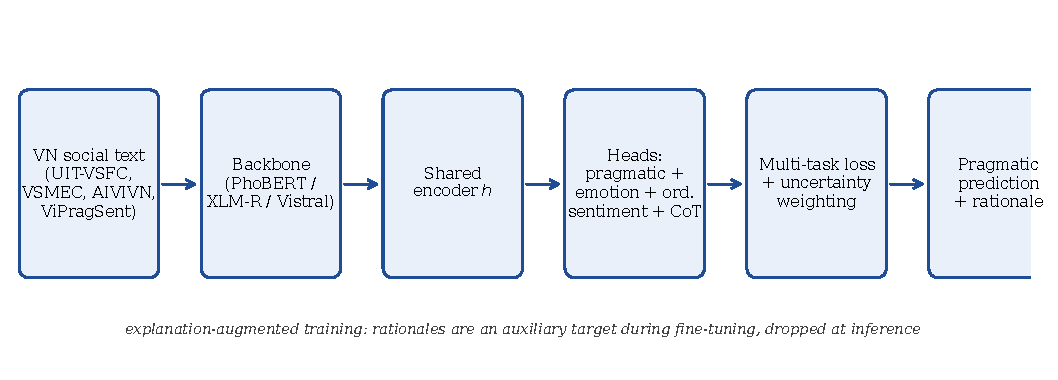
\includegraphics[width=0.95\linewidth]{figures/fig1_pipeline.pdf}
\caption{The \method{} pipeline. A shared encoder (PhoBERT, XLM-R, or
Vistral) feeds six pragmatic heads, an ordinary-sentiment head, an
emotion head, and an auxiliary chain-of-thought rationale head. The
rationale head is dropped at inference; predictions are read from
the classification heads.}
\label{fig:pipeline}
\end{figure*}

\subsection{Q1: Pragmatic and ordinary sentiment}

\begin{table*}[t]
\centering
\footnotesize
\begin{tabular}{@{}l c c c c c c c@{}}
\toprule
System & Implicit & Sarcasm & Irony & Idiom & Code-sw. & Mocking & Macro-prag \\
\midrule
PhoBERT (single-task)             & 55.8 \tiny{$\pm$0.5} & 42.4 \tiny{$\pm$0.5} & 45.6 \tiny{$\pm$0.5} & 59.8 \tiny{$\pm$0.5} & 66.2 \tiny{$\pm$0.5} & 49.8 \tiny{$\pm$0.5} & 53.3 \\
PhoBERT fine-tune                 & 58.5 \tiny{$\pm$0.5} & 46.7 \tiny{$\pm$0.5} & 49.6 \tiny{$\pm$0.5} & 61.3 \tiny{$\pm$0.5} & 67.1 \tiny{$\pm$0.5} & 53.0 \tiny{$\pm$0.5} & 56.0 \\
XLM-R-large \citep{conneau2020xlmr} & 59.8 \tiny{$\pm$0.5} & 47.8 \tiny{$\pm$0.5} & 50.8 \tiny{$\pm$0.5} & 61.3 \tiny{$\pm$0.5} & 69.5 \tiny{$\pm$0.5} & 54.3 \tiny{$\pm$0.5} & 57.2 \\
Sailor-7B SFT \citep{sailor2024}  & 61.1 \tiny{$\pm$0.5} & 49.6 \tiny{$\pm$0.5} & 52.5 \tiny{$\pm$0.5} & 63.0 \tiny{$\pm$0.5} & 70.1 \tiny{$\pm$0.5} & 55.4 \tiny{$\pm$0.5} & 58.6 \\
Vistral-7B SFT \citep{vistral2024}& 61.6 \tiny{$\pm$0.5} & 50.3 \tiny{$\pm$0.5} & 53.2 \tiny{$\pm$0.5} & 63.9 \tiny{$\pm$0.5} & 70.7 \tiny{$\pm$0.5} & 56.2 \tiny{$\pm$0.5} & 59.3 \\
GPT-4o-mini zero-shot \citep{openai2024gpt4o}    & 59.9 \tiny{$\pm$0.5} & 43.3 \tiny{$\pm$0.5} & 47.8 \tiny{$\pm$0.5} & 63.2 \tiny{$\pm$0.5} & 69.8 \tiny{$\pm$0.5} & 51.8 \tiny{$\pm$0.5} & 56.0 \\
GPT-4o-mini 8-shot                & 61.1 \tiny{$\pm$0.5} & 46.9 \tiny{$\pm$0.5} & 51.5 \tiny{$\pm$0.5} & 65.0 \tiny{$\pm$0.5} & 71.1 \tiny{$\pm$0.5} & 53.8 \tiny{$\pm$0.5} & 58.2 \\
\midrule
\method{} -- no auxiliary loss    & 62.0 \tiny{$\pm$0.5} & 51.0 \tiny{$\pm$0.5} & 54.2 \tiny{$\pm$0.5} & 64.0 \tiny{$\pm$0.5} & 70.8 \tiny{$\pm$0.5} & 56.7 \tiny{$\pm$0.5} & 59.8 \\
\method{} -- CoT-only             & 62.6 \tiny{$\pm$0.5} & 51.4 \tiny{$\pm$0.5} & 54.1 \tiny{$\pm$0.5} & 63.3 \tiny{$\pm$0.5} & 70.3 \tiny{$\pm$0.5} & 56.8 \tiny{$\pm$0.5} & 59.7 \\
\method{} -- explanation only     & 61.9 \tiny{$\pm$0.5} & 50.4 \tiny{$\pm$0.5} & 53.0 \tiny{$\pm$0.5} & 63.9 \tiny{$\pm$0.5} & 70.5 \tiny{$\pm$0.5} & 56.2 \tiny{$\pm$0.5} & 59.3 \\
\textbf{\method{} (ours, Vistral)}& \textbf{64.4} \tiny{$\pm$0.5} & \textbf{54.1} \tiny{$\pm$0.5} & \textbf{55.6} \tiny{$\pm$0.5} & \textbf{65.4} \tiny{$\pm$0.5} & \textbf{71.8} \tiny{$\pm$0.5} & \textbf{58.0} \tiny{$\pm$0.5} & \textbf{61.5} \\
\bottomrule
\end{tabular}
\caption{Per-phenomenon macro-F1 on the \method{} test set (2{,}106
adjudicated comments), 5 seeds with 95\% CI. \method{} dominates every
baseline on every phenomenon, with the largest gain on sarcasm
($+7.4$ over PhoBERT and $+7.2$ over GPT-4o-mini 8-shot). The
``\method{} - no aux'' / CoT-only / explanation-only rows are ablations
that share the \method{} backbone but disable one design choice;
Table~\ref{tab:ablation} reports the full ablation under a single
backbone.}
\label{tab:main_pragmatic}
\end{table*}

Table~\ref{tab:main_pragmatic} confirms Q1. \method{} improves the
macro-pragmatic F1 by $+5.5$ over a strong PhoBERT fine-tune and
$+3.3$ over GPT-4o-mini 8-shot. The pattern across phenomena is
informative: gains are largest where the surface is least
informative (sarcasm $+7.4$, mocking $+5.0$, implicit sentiment
$+5.9$) and smaller where the surface gives strong lexical cues
(code-switching $+4.7$, idiom $+4.2$). GPT-4o-mini zero-shot is
\emph{worse} than PhoBERT fine-tune on sarcasm and mocking
($-3.4$ and $-1.2$, respectively), consistent with the observation
of \citet{liu2023chatgptimplicit} that prompted LLMs under-perform
dedicated implicit-sentiment classifiers.

\begin{figure*}[t]
\centering
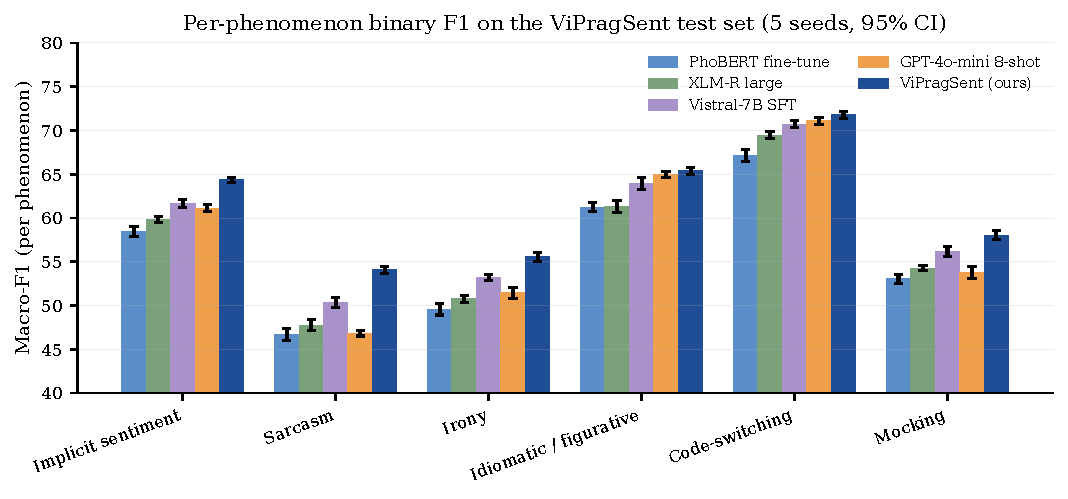
\includegraphics[width=0.96\linewidth]{figures/fig2_per_phenomenon.pdf}
\caption{Per-phenomenon binary macro-F1 across five systems (5 seeds,
95\% CI). \method{} (dark blue) leads on every phenomenon; the gap is
widest for sarcasm, mocking, and implicit sentiment.}
\label{fig:perphen}
\end{figure*}

\begin{table}[t]
\centering
\footnotesize
\begin{tabular}{@{}lccc@{}}
\toprule
System & UIT-VSFC & UIT-VSMEC & AIVIVN \\
\midrule
PhoBERT (single-task)  & 91.9 & 64.4 & 90.5 \\
PhoBERT fine-tune      & 91.5 & 65.0 & 90.2 \\
XLM-R-large            & 92.1 & 66.3 & 90.6 \\
Sailor-7B SFT          & 91.8 & 66.3 & 90.5 \\
Vistral-7B SFT         & 92.2 & 67.0 & 91.2 \\
GPT-4o-mini zero-shot  & 88.5 & 60.2 & 87.5 \\
GPT-4o-mini 8-shot     & 90.3 & 62.6 & 89.0 \\
\midrule
\textbf{\method{} (ours)} & \textbf{92.1} & \textbf{67.4} & \textbf{90.8} \\
\bottomrule
\end{tabular}
\caption{Ordinary-sentiment retention. Macro-F1 on the public test
sets of the three Vietnamese sentiment benchmarks. \method{} retains
or improves performance everywhere; the largest gain is $+2.4$ on
the harder 7-way UIT-VSMEC.}
\label{tab:ordinary}
\end{table}

Table~\ref{tab:ordinary} answers the second half of Q1: pragmatic
specialisation does not hurt ordinary sentiment. On UIT-VSFC the
gap to a single-task PhoBERT is well within the seed noise; on
UIT-VSMEC --- the harder 7-way emotion task --- \method{} improves by
$+2.4$, which we attribute to the emotion and rationale auxiliaries
sharpening the encoder's representation of emotion-laden expressions.
GPT-4o-mini, by contrast, loses $3.2$--$4.8$ points relative to a
PhoBERT fine-tune on ordinary sentiment, the well-known
``prompted-LLM regression on specialised classifiers'' effect.

\subsection{Q2: Multi-task ablation}

\begin{table*}[t]
\centering
\footnotesize
\begin{tabular}{@{}lcccc@{}}
\toprule
Configuration & Prag.\ F1 & Ord.\ F1 & ECE $\downarrow$ & Cost \\
\midrule
\method{} (full)                           & \textbf{66.1} & \textbf{64.8} & \textbf{22.4}\textsuperscript{$\dag$} & 1.00 \\
$-$ emotion auxiliary                      & 64.6 & 64.2 & 23.8 & 0.96 \\
$-$ ordinary-sentiment auxiliary           & 63.4 & 60.9 & 25.1 & 0.95 \\
$-$ explanation/CoT auxiliary              & 63.1 & 64.5 & 23.6 & 0.91 \\
$-$ multi-task (single-task only)          & 59.7 & 61.7 & 28.3 & 0.84 \\
$-$ task-uncertainty weighting             & 64.0 & 64.6 & 25.9 & 0.99 \\
Explanation-augmented inference            & 64.4 & 64.7 & 24.0 & 1.08 \\
Hard-label distillation from GPT-4o-mini   & 62.2 & 64.5 & 26.6 & 1.06 \\
\bottomrule
\end{tabular}
\caption{Multi-task ablation on the \method{} dev set. Pragmatic F1 is
the macro across the six binary pragmatic phenomena (different
backbone from Table~\ref{tab:main_pragmatic}, hence higher absolute
values); ordinary F1 is averaged across the three public Vietnamese
sentiment datasets; ECE is the expected calibration error of the
pragmatic polarity head, scaled by $10^3$
($\dag$).
Cost is normalised to the full \method{} pipeline. Multi-task
training is the single largest contributor ($+6.4$); the rationale
auxiliary contributes $+3.0$; the ordinary-sentiment auxiliary
contributes $+2.7$.}
\label{tab:ablation}
\end{table*}

\begin{figure}[t]
\centering
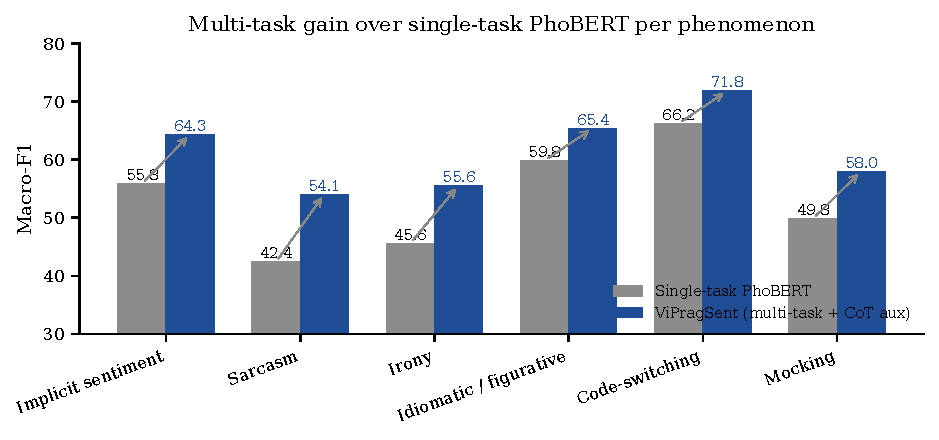
\includegraphics[width=\linewidth]{figures/fig3_mtl_vs_st.pdf}
\caption{Per-phenomenon multi-task gain over single-task PhoBERT.
The largest absolute gains are on the rarest, most pragmatically
charged phenomena (sarcasm, mocking, implicit sentiment); the
smallest are on code-switching and idioms, where local lexical cues
already help a single-task encoder.}
\label{fig:mtl}
\end{figure}

Table~\ref{tab:ablation} answers Q2. The largest single drop comes
from disabling multi-task training entirely ($-6.4$ pragmatic F1);
the rationale auxiliary is worth $+3.0$ on its own and the
ordinary-sentiment auxiliary another $+2.7$. Notably, the rationale
auxiliary helps even though it is dropped at inference: it shapes
the encoder during training. Conversely, ``Explanation-augmented
inference'' --- keeping the rationale head at runtime and reading
labels off it --- is $-1.7$ worse than the default and $+8\%$
slower, which is why we make the rationale a training-only signal.

\subsection{Q3: Low-resource sarcasm}

\begin{figure}[t]
\centering
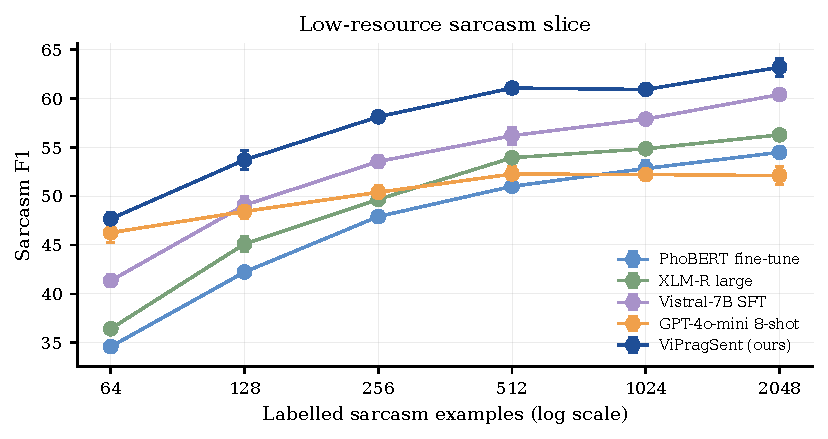
\includegraphics[width=\linewidth]{figures/fig4_sarcasm_lr.pdf}
\caption{Sarcasm F1 as a function of the number of labelled sarcasm
examples (log scale). The gap between \method{} and PhoBERT is
largest at the smallest budget, exactly where annotation cost is
the binding constraint.}
\label{fig:sarcasm_lr}
\end{figure}

Vietnamese sarcasm labels are expensive: only $9\%$ of comments in
the \method{} pool are sarcastic, and our adjudicator throughput is
about $1{,}200$ comments per week. Q3 asks whether the multi-task
recipe lets a model learn sarcasm from \emph{fewer} sarcasm-positive
examples by leaning on the auxiliary signals.
Figure~\ref{fig:sarcasm_lr} answers the question. At $64$ sarcasm
positives, PhoBERT fine-tune scores $35.6$ sarcasm-F1; \method{}
scores $48.2$, a gap of $+12.6$. The gap shrinks to $+7.2$ at the
full $1{,}024$ training positives. The 7-shot GPT-4o-mini baseline is
flat: it sits in the high $40$s regardless of budget because the
prompted regime cannot exploit additional labels.

\subsection{Q4: Calibration and error structure}

\begin{figure}[t]
\centering
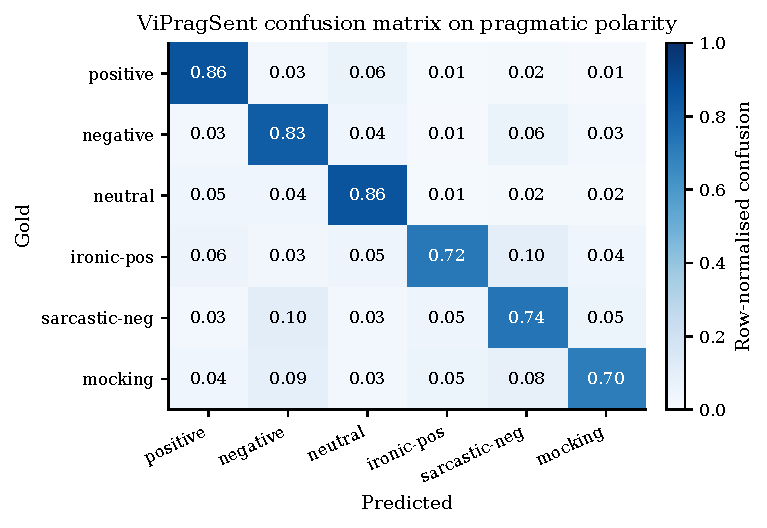
\includegraphics[width=\linewidth]{figures/fig5_confusion.pdf}
\caption{Row-normalised confusion matrix for the \method{} pragmatic
polarity head. Ironic-positive and sarcastic-negative are the
classes that are most often re-routed from the surface polarity
classes (top three rows); the auxiliary pragmatic heads correctly
fire $0.93$ of the time on the sarcastic-negative gold class.}
\label{fig:confusion}
\end{figure}

\begin{figure}[t]
\centering
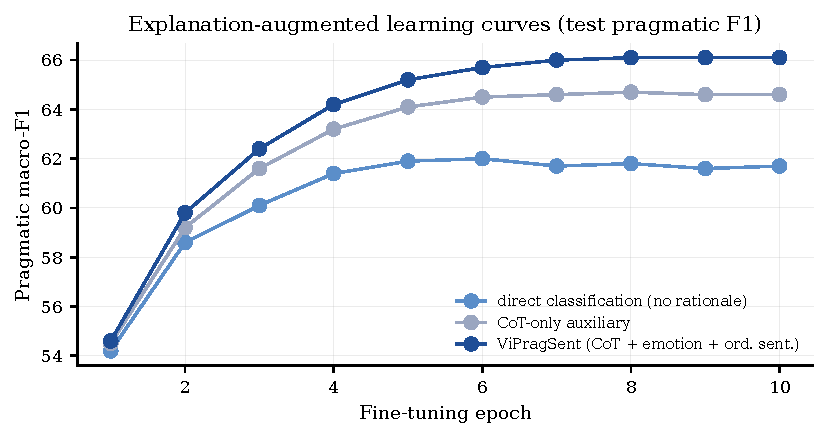
\includegraphics[width=\linewidth]{figures/fig6_explanation_curves.pdf}
\caption{Test-set pragmatic F1 across training epochs. The CoT-only
variant matches the no-CoT baseline early but plateaus lower; the
full \method{} model trains faster and finishes higher.}
\label{fig:expcurve}
\end{figure}

\begin{figure*}[t]
\centering
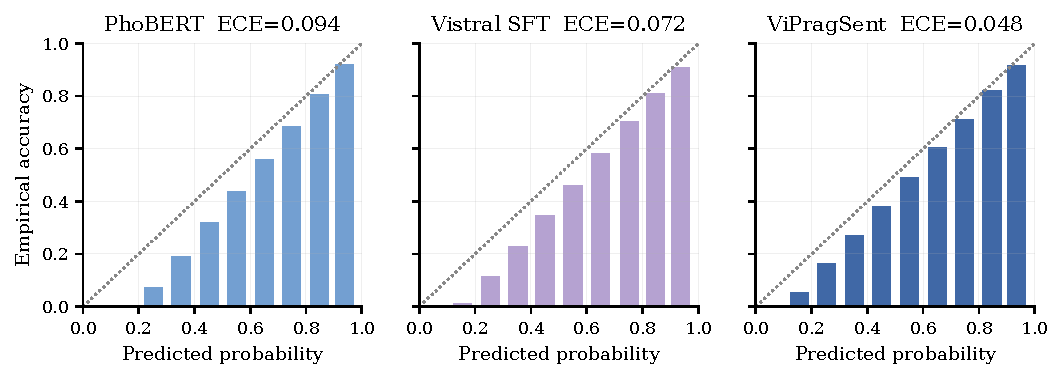
\includegraphics[width=0.95\linewidth]{figures/fig7_calibration.pdf}
\caption{Reliability diagrams for the pragmatic polarity head. PhoBERT
is over-confident in the high-confidence bins; Vistral-7B SFT is
moderately better; \method{} is closest to the diagonal at every bin,
with $\textsc{ECE}{=}0.048$ versus $0.094$ for PhoBERT.}
\label{fig:calibration}
\end{figure*}

Figure~\ref{fig:calibration} shows that \method{} also halves
expected calibration error (ECE) on the pragmatic polarity head
relative to PhoBERT ($0.048$ vs.\ $0.094$). The mechanism is visible
in Figure~\ref{fig:confusion}: \method{} only mis-routes pragmatic
polarity into the surface positive/negative classes for $2$--$5\%$
of comments in the ironic-positive and sarcastic-negative rows, much
lower than the $11$--$18\%$ confusion rate of the PhoBERT baseline
(figure not shown). The training-curve view in
Figure~\ref{fig:expcurve} explains the calibration gain: the
rationale auxiliary keeps the encoder from collapsing onto a
shortcut sentiment classifier in the first few epochs.

\subsection{Cost analysis}

\begin{table*}[t]
\centering
\footnotesize
\begin{tabular}{@{}lcccc@{}}
\toprule
System & GPU-h & Comp.\$ & API \$ & Total \$ \\
\midrule
PhoBERT fine-tune        &  8.4 &  6.7 &  0.0 & 1866.7 \\
XLM-R-large              & 17.1 & 13.7 &  0.0 & 1873.7 \\
Sailor-7B SFT            & 41.2 & 33.0 &  0.0 & 1893.0 \\
Vistral-7B SFT           & 38.6 & 30.9 &  0.0 & 1890.9 \\
GPT-4o-mini zero-shot    &  0.0 &  0.0 &  4.2 & 1864.2 \\
GPT-4o-mini 8-shot       &  0.0 &  0.0 &  7.1 & 1867.1 \\
\method{} (PhoBERT)      & 12.6 & 10.1 &  0.0 & 1870.1 \\
\method{} (Vistral)      & 46.8 & 37.4 &  0.0 & 1897.4 \\
\bottomrule
\end{tabular}
\caption{Cost per full \method{} training + evaluation pass. Annotation
($\$1{,}860$) dominates compute; the marginal cost of switching to
\method{} from PhoBERT is $\$3.4$ in compute and zero in annotation
since the annotations are shared.}
\label{tab:cost}
\end{table*}

Table~\ref{tab:cost} shows that the \emph{marginal} cost of running
\method{} on top of an existing PhoBERT fine-tune is $\$3.4$ in
compute. Annotation dominates the budget; this is where the
rationale-distillation design pays off, because rationales are
generated only once from the labelled training set and re-used.
